\documentclass{article}
\usepackage{graphicx}
\usepackage{subcaption}
\begin{document}
	\section{Motivation}
	The programming language is python. The basic algorithm is the nearest centroid mean algorithm. The algorithm initially compute the mean for each class. The mean is a vector which is computed by averaging two features of training data. The algorithm to classify data is to compute the Euclidean distance between feature vector and  mean vector trained by the classifier. 
	
	\section{Problem solution}
	\subsection{problem a}
	Two figures are generated by using \textit{PlotDecBoundaries()}. The CSV file is read by the library supported by the numpy. The data is stored into the \textit{ndarray}.  The Figure \ref{fig:synthetictrain1} shows the data points, class mean and decision boundary for synthetic data set 1. The Figure \ref{fig:synthetictrain2} shows these information for synthetic data set 2. 
	\begin{figure}[hbt!]
		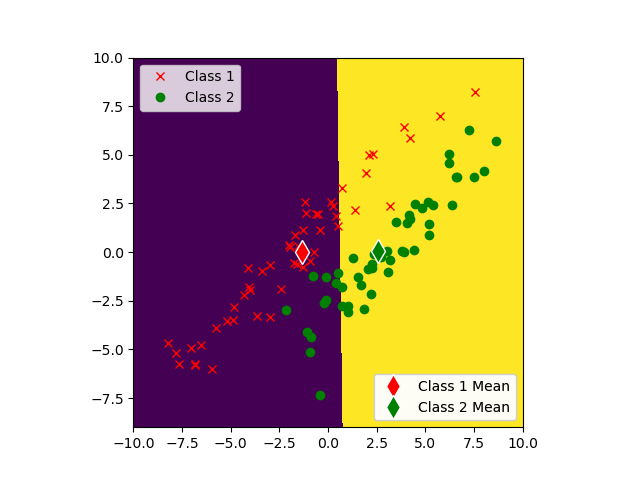
\includegraphics[width=\linewidth]{images/synthetic_trian1.png}	
		\caption{synthetic train1}
		\label{fig:synthetictrain1}
	\end{figure}
	\begin{figure}[hbt!]
		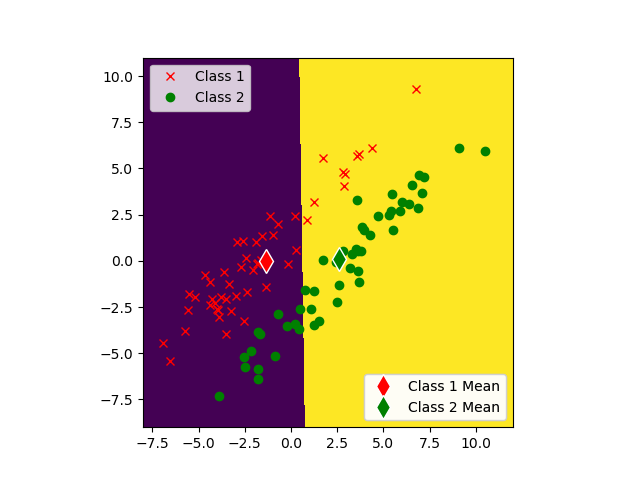
\includegraphics[width=\linewidth]{images/synthetic_test1.png}
		\caption{synthetic test1}
		\label{fig:synthetictest1}
	\end{figure}
	\begin{figure}[hbt!]
		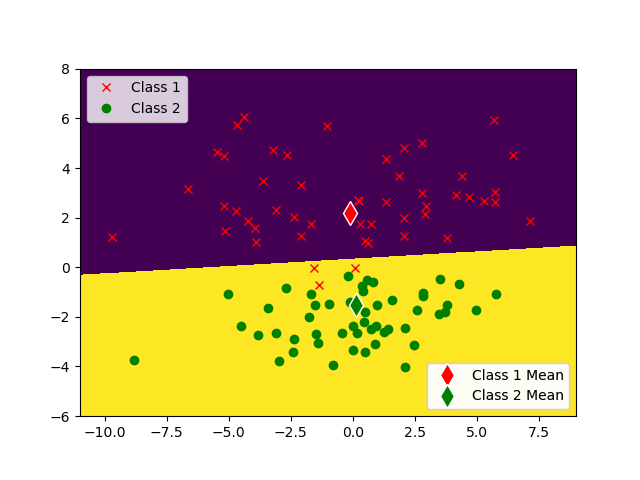
\includegraphics[width=\linewidth]{images/synthetic_train2.png}
		\caption{synthetic train2}
		\label{fig:synthetictrain2}
	\end{figure}
	\begin{figure}[hbt!]
		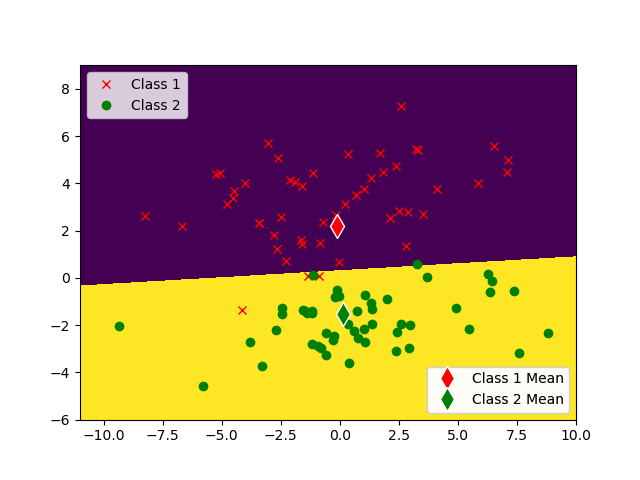
\includegraphics[width=\linewidth]{images/synthetic_test2.png}
		\caption{synthetic test2}
		\label{fig:synthetictest2}
	\end{figure}
		\begin{table}[hbt!]
		\begin{center}
		\begin{tabular}{| l | l | l | p{5cm} |}
		\hline
			Data      & Error rate & Test samples  \\ \hline
			synthetictrain1& 0.24        & 100    \\  \hline
			synthetictest1& 0.24		& 100    \\   \hline
			synthetictrain2& 0.04        & 100    \\  \hline
			synthetictest2& 0.04		& 100    \\   \hline
		\end{tabular}
		\end{center}
	\caption{Error rate}
	\label{table: errorrate}
	\end{table}
	 \\
	\subsection{problem b}
	The error rate of both synthetic data set is shown in the table \ref{table: errorrate}. The table also shows the error rate of the synthetic data set 2 is smaller than the error rate of the synthetic data set 1. The performance of data set 2 is also good in the training data set. The class error is computed by running python program synthetic.py. The console display the error rate. 
	\subsection{problem c}
		\begin{figure}[hbt!]
		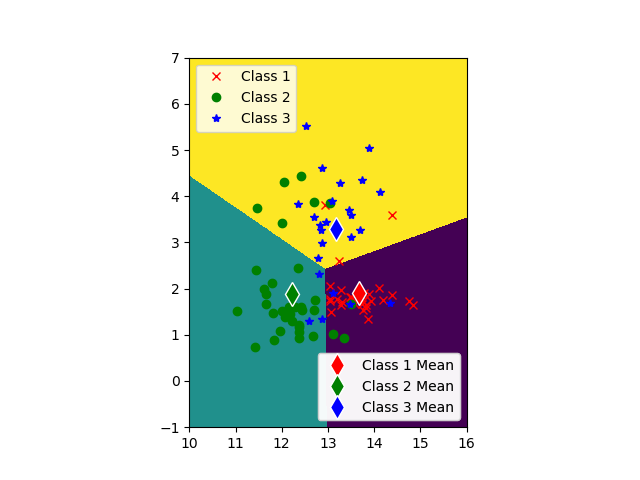
\includegraphics[width=\linewidth]{images/wine_feature01_train.png}	
		\caption{the data scatter plot of wine data set whose feature is 0 and 1}
		\label{fig:wine_feature01_train}
	\end{figure} 
	The Figure \ref{fig:wine_feature01_train} shows the training data points, sample mean and decision boundary for wine data set. 
	\subsection{problem d}
		\begin{table}[hbt!]
		\begin{center}
			\begin{tabular}{| l | l | l | l | l | p{5cm} |}
				\hline
				ID     & Error rate(Train Data) & Error rate(Test Data) & Feature1 & Feature2   \\ \hline
				1      & 0.11     &    2   & 100      &   1         \\      \hline
				2      & 0.24	  &	    3  & 100      &    2        \\      \hline
				3      & 0.04     &      4 & 100      &     2       \\      \hline
				4      & 0.04	  &	      5& 100      &      2      \\      \hline
			\end{tabular}
		\end{center}
		\caption{Error rate for wine data set}
		\label{table: errorrate}
	\end{table}
	The method to sdf
	\subsection{problem e}
	\section{Summary}
	
\end{document}